\documentclass[12pt, a4paper]{report}

%dvips OR pdftex
\usepackage[pdftex, pdfauthor={YKY}, bookmarks, anchorcolor=blue, colorlinks, linkcolor=blue, citecolor=blue, urlcolor=blue, breaklinks, plainpages=false, pdfpagelabels, hypertexnames=false]{hyperref}
\usepackage{breakurl}
\usepackage[final]{graphicx}
\usepackage{float}
\usepackage[square]{natbib}
\usepackage{color}
\usepackage{amsmath}     % for {equation} {cases} {xleftarrow}
\usepackage{bbm}         % for math fonts with double lines
\usepackage{amssymb}     % for \curlyvee
\usepackage{stmaryrd}    % for \bigcurlyvee, \widetilde{\bigwedge}
\usepackage{wasysym}     % for \iint (double integral)
\usepackage{makeidx}
\usepackage[style=list,acronym=true,number=none]{glossary}
\usepackage{alg}
\usepackage{minitoc}
\usepackage[sf,bf,big,raggedright,compact]{titlesec}
\usepackage{fancyhdr}
\usepackage{movie15}
\usepackage{caption}
\usepackage{parskip}     % may not need
\usepackage[pointedenum]{paralist}  % compactenum, compactitem etc
\usepackage{enumitem}    % fixes para top seperation in {enumerate}
\setlist{topsep=-1ex}
\usepackage{amsthm}      % theorem style

%\newenvironment{compactitem}[0]{\begin{enumerate}[label=\textbullet,noitemsep]}{\end{enumerate}}

\newenvironment{compactenum-}[0]{\begin{compactenum}}{\end{compactenum}\vspace{3ex}}
\newenvironment{compactitem-}[0]{\begin{compactitem}}{\end{compactitem}\vspace{3ex}}
\newenvironment{enumerate-}[0]{\begin{enumerate}}{\end{enumerate}\vspace{3ex}}

%\newenvironment{compactenuma}[0]{\begin{enumerate}[nosep,label=\alpha]}{\end{enumerate}}

\definecolor{TodoColor}{rgb}{0.1,0.4,0.1}   % Dark Green
\definecolor{LogicColor}{rgb}{0.4,0.1,0.4}  % Magenta
\definecolor{Green} {rgb}{0.1,0.4,0.1}
\definecolor{Red}   {rgb}{1.0,0.4,0.4}
\definecolor{Blue}  {rgb}{0.1,0.1,0.6}
\definecolor{Purple}{rgb}{0.4,0.1,0.3}

\newcommand{\code}   [1]{{\footnotesize{\ttfamily #1}}}
\newcommand{\formula}[1]{\textcolor{LogicColor}{#1}}
\newcommand{\todo}   [1]{\textcolor{TodoColor}{\{ #1 \}}}
\newcommand{\english}[1]{\rmfamily \textit{``#1''}\sffamily}
\newcommand{\kb}     [1]{[s$_#1$]:}
\renewcommand{\star}{$* \;$}
\newcommand{\app}{$\circ \;$}
\newcommand{\eg}{\textbf{Example:} }
\newcommand{\tab}{\hspace*{1cm} }
\renewcommand{\vec}[1]{\mathbf{#1}}

\newcommand{\underconst}{
\includegraphics[scale=0.5]{UnderConst.png}}

%%%%%%%%%%%%%%%%% Symbols defined by me %%%%%%%%%%%%%%%%%%%
\newcommand{\defeq}{\stackrel{def}{=}}
% fuzzy and probabilistic logic operators
\newcommand{\tv}[1]{$\langle${#1}$\rangle$}
\newcommand{\Zand}{\stackrel{Z}{\wedge}}
\newcommand{\Zor}{\stackrel{Z}{\vee}}
\newcommand{\Zneg}{\stackrel{Z}{\neg}}
\newcommand{\Pand}{\stackrel{P}{\wedge}}
\newcommand{\Por}{\stackrel{P}{\vee}}
\newcommand{\bigZand}{\stackrel{Z}{\bigwedge}}
\newcommand{\bigZor}{\stackrel{Z}{\bigvee}}
\newcommand{\bigPand}{\stackrel{P}{\bigwedge}}
\newcommand{\bigPor}{\stackrel{P}{\bigvee}}
\newcommand{\Pandor}{\stackrel{P}{\varodot}}
\newcommand{\Zandor}{\stackrel{Z}{\varodot}}
\newcommand{\bigPandor}{\stackrel{P}{\bigodot}}
\newcommand{\bigZandor}{\stackrel{Z}{\bigodot}}
\newcommand{\Pimp}{\rightarrowtriangle}       % probabilistic implication ->
\newcommand{\PimpL}{\leftarrowtriangle}       % probabilistic implication <-
% categories
\newcommand{\catP}{\mathcal{P}}
\newcommand{\catZ}{\mathcal{Z}}
\newcommand{\catB}{\mathcal{B}}
\newcommand{\catC}{\mathcal{C}}
\newcommand{\catPB}{\mathcal{P(B)}}
\newcommand{\catPZ}{\mathcal{P(Z)}}
\newcommand{\setN}{\mathbb{N}}
\newcommand{\setR}{\mathbb{R}}
\newcommand{\Hyp}{\mathbbm{Hyp}}

\fontsize{13pt}{15pt} \selectfont
\renewcommand{\familydefault}{\sfdefault}
%\renewcommand{\mtcfont}{\small\sffamily}
%\renewcommand{\mtcSfont}{\small\sffamily}
%\renewcommand{\mtcSSfont}{\small\sffamily}
%\renewcommand{\mtcSSSfont}{\small\sffamily}
%\renewcommand{\mtifont}{\small\sffamily}
\renewcommand{\mtcfont}{\normalsize\sffamily}
\renewcommand{\mtcSfont}{\normalsize\sffamily}
\renewcommand{\mtcSSfont}{\normalsize\sffamily}
\renewcommand{\mtcSSSfont}{\normalsize\sffamily}
\renewcommand{\mtifont}{\normalsize\sffamily}
%\renewcommand{\mtcfont}{\large\sffamily}
%\renewcommand{\mtcSfont}{\large\sffamily}
%\renewcommand{\mtcSSfont}{\large\sffamily}
%\renewcommand{\mtcSSSfont}{\large\sffamily}
%\renewcommand{\mtifont}{\large\sffamily}
\renewcommand{\mtctitle}{}
\renewcommand{\chaptername}{Ch }

\newtheoremstyle{examples}{}{}{\upshape}{}{\bfseries}{}{\newline}{#1 #2 \mdseries{#3}}
\theoremstyle{examples} \newtheorem{example}{Example}[section]

\titlespacing{\chapter}{0pt}{0pt}{0pt}
\titleformat{\chapter}[hang]{\sffamily\bfseries\Huge\color{blue}}{\thechapter \hspace{30pt}}{0pt}{}
\titleformat{\appendix}[hang]{\sffamily\bfseries\Huge\color{blue}}{\thechapter \hspace{30pt}}{0pt}{}
\titleformat{\section}[hang]{\sffamily\bfseries\Large\color{blue}}{\thesection \hspace{10pt}}{0pt}{}
\titleformat{\subsection}[hang]{\sffamily\bfseries\large\color{blue}}{\thesubsection \hspace{5pt}}{0pt}{}
\titleformat{\subsubsection}[hang]{\sffamily\bfseries\color{blue}}{\thesubsubsection \hspace{5pt}}{0pt}{}

\newcommand{\algrepeatforever}{\textbf{repeat forever}\\\algbegin}

\interfootnotelinepenalty=50000

\title{\textbf{Genifer\\-- an artificial general intelligence}}
\author{YKY (general.intelligence@Gmail.com)\\ \\
with input from:\\
Abram Demski\\
Ben Goertzel\\
Martin Magnusson\\
Russell Wallace\\
Pei Wang
}
\date{\copyright \quad latest revision: \today}

\setlength{\headheight}{0cm}
\setlength{\hoffset}{0cm}
\setlength{\topmargin}{-2cm}
\setlength{\oddsidemargin}{-2cm}
\setlength{\evensidemargin}{-2cm}
\setlength{\textwidth}{19.5cm}
\setlength{\textheight}{28cm}
\setlength{\headsep}{0cm}
\setlength{\topskip}{0cm}
\setlength{\footskip}{0.9cm}  % between bottom of page and page number
\setlength{\floatsep}{0cm}
\setlength{\textfloatsep}{0.6cm}
\setlength{\intextsep}{0.5cm}
\setlength{\parindent}{0em}   % em = width of capital M
\setlength{\parskip}{2ex plus1ex minus1ex} % ex = height of lowercase letter x
% \setlength{\topsep}{-1ex}
\setlength{\pltopsep}{-3ex}   % for compact-enum

\pagestyle{fancy}
\renewcommand{\headrulewidth}{0pt}
\rhead{}
\lhead{}
\cfoot{}
\rfoot{\thepage}
\fancypagestyle{plain}{\rfoot{\thepage}}
%\pagestyle{plain}

\includeonly{introduction, architecture, knowledge-representation, logic, vagueness, probabilities, confidence, inference, pattern-recognition, belief-revision, induction, natural-language, memory-systems, planning, program-synthesis, value-judgements, vision, implementation, business-aspects, quick-start, symbols}

\makeindex
\makeglossary

\begin{document}
%\font\normalfont=cmss14
\renewcommand{\normalsize}{\fontsize{13pt}{15pt}\selectfont}
\fontsize{13pt}{15pt} \selectfont

%\pagestyle{plain}
%\newcommand\ps@plain{
%\renewcommand\@oddhead{}
%\let\@evenhead\@oddhead
%\renewcommand\@evenfoot
%    {\hfil{\thepage}}
%\let\@oddfoot\@evenfoot
%}

\maketitle
\dominitoc

\setcounter{chapter}{-1}
\chapter{Preface and to-do list}

\begin{enumerate}

\item  This book is a perpetual draft.

\item  My personal reason for developing AGI is to achieve life extension.

\item  The source code of $\mbox{Genifer}$ is hosted on \href{http://code.google.com/p/genifer/}{Google Code}, including some very easy \href{http://code.google.com/p/genifer/downloads/list}{tutorial slides}.  Also feel free to \href{mailto:Generic.Intelligence@Gmail.com}{contact me}!

\end{enumerate}

\begin{flushright}
--- YKY
\end{flushright}

\color{TodoColor}

{\sffamily\bfseries\Huge To-do:}

\begin{description}

\item[Ch 1 (Introduction)]  Explain the new ideas that I learned about the relationship between propositional logic and topological logic.

\item[Ch 2 (Architecture)]  Explain AIXI, algorithmic complexity, Solomonoff induction, etc.  Explain my distributive architecture.

\item[Ch 3 (KR)] --- ok ---

\item[Ch 4 (Logic)]  New idea about equational unification and concepts.  Explain background notions, eg paradoxes.

\item[Ch 5 (Z)]  Add new idea on the ``Java-girl paradox'', which is in my draft paper.

\item[Ch 8 (Inference)]  Copy and paste Bayesian inference and factor graph stuff from the Lisp code to here.

\item[Ch 9 (Pattern recognition)]  Brush up the definition of the similarity relation.

\item[Ch 11 (Learning)]  A lot of new material is in the slides.

\item[Ch 12 (NL)] --- ok ---

\item[Ch 13 (Memory)]  Explain hierarchical clustering idea (from slides).

\item[Ch 14 (Planning)]  May need re-think.

\item[Appendix A]  Recommend more books for AGI sub-areas.  Especially math books.

\end{description}

%end of to-do
\color{black}

\tableofcontents

\include{introduction}
\include{architecture}
\chapter{Knowledge representation}
\minitoc

\section{Introduction}

An AGI uses a KR structure to \textit{represent} the external world, and this structure is built with limited computational resources, and as such, must be approximate.  We have a lot of freedom to choose the KR format.

I chose logic as KR because it offers a \textit{direct} way to translate natural-language texts into machine knowledge.  This is of critical importance because the overall feasibility of AGI hinges on the efficiency of machine learning, and the most effective machine-learning method is ``learn by being told'' (\S\ref{sec:learn-by-being-told}).

A common misconception is:  ``How can complex ideas such as `John loves Mary' be reduced to logic formulae like \textit{loves(john,mary)}?''  One school of thought (see eg \citep*{Johnson-Laird1983}) posits that human reasoning is based on ``mental models'', but it is unclear how exactly they can be constructed.  My view of logic-based AI is that of using logic as a \textit{computational structure} for \textit{constructing} mental models.

% Sorted or unsorted logic?

\section{Natural language}

Please also see the chapter on natural language (\ref{ch:natural-language}).

\subsection{Composition of concepts}
\label{sec:composition}

In 1928 the young Haskell Curry started working on \textbf{combinatory logic} (CL) as a \textit{logica universalis}, but it ran into inconsistency problems \footnote{In Genifer we try to use fuzzy-probabilistic truth values to get around this problem (see \S\ref{sec:paradox}).}.  One special feature of CL is \textbf{combinatorial completeness} -- meaning that any concept can, in principle, be applied to any other concept.  One can readily see that, when the concept of \textit{self-application} is applied to itself, it can lead to Russell's paradox (\S\ref{sec:paradox}).

Nevertheless, combinatorial completeness is something desirable in a universal logic.  It enables a logic to \textit{reason about logical paradoxes themselves}.  Bertrand Russell invented \textbf{type theory} to get around the problem of paradoxes, basically by banning all circular references.  But as a result of that, type theory (and thus the higher-order logic built on top of it) cannot be used to reason about paradoxes.

Curry's combinatory logic can represent arbitrary combinations of concepts, in a manner such as:\\
\tab $\lceil$wisdom$\rceil$ $\bullet$ $\lceil$socrates$\rceil$ = $\lceil$the wisdom of socrates$\rceil$

One of my latest insights is that the combination of concepts can be computed by the same process as \textbf{unification} of terms in logic.  For more details, refer to \S\ref{sec:unification}.

In 1963 JA Robinson discovered resolution, which is really unification + propositional refutation.  Unification decides if 2 terms can be made equationally identical.  Propositional refutation is an inference step that deals with the "calculus of thinking" at the \textit{sentence} level.

Around the 1900s, George Boole, CS Peirce, Gottlob Frege, amongst others, developed \textbf{predicate logic}, which is later popularized by people such Hilbert, Ackermann, Russell, and Whitehead.  Predacate logic has really been popular for only about 80 years, versus syllogistic logic that has been around since Aristotle's time.  Predicate logic differs from propositional logic by giving propositions \textit{internal structure} -- a proposition is broken down into a \textbf{predicate} and one or more \textbf{objects}.  However, this decomposition seems inadequate to deal with arbitrarily free combinations of concepts.

Combinatory logic provides a free way to compose terms via "application".  The key is to regard terms as (compound) concepts.  For example, in Genifer's notation:\\
\tab "tall handsome guy"\\
is the combination of the concepts\\
\tab (tall, handsome) $\circ$ guy.

Now, a few examples:\\
"tall handsome guy" is equivalent to "handsome tall guy";\\
"very tall guy" implies "tall guy";  but\\
"very tall guy" does not equal "tall very guy";

Thus the unification is modulo some special rules such as commutativity, associativity, etc, and certain reduction rules.  In other words, unification modulo a theory = "the calculus of concepts".

So we have a neat decomposition:\\
\tab calculus of thoughts = calculus of concepts + calculus of propositions

In \textbf{category theory}, one enforces the associative composing of arrows:\\
\tab $(ab)c = a(bc)$. \footnote{We often omit the application symbol $\circ$.}\\
Likewise, I observed that if we enforce the associative composition of concepts, the logical form becomes very elegant.  Due to associativity, any pair of concepts in an application:\\
\tab $a \circ b$\\
must be \textit{meaningful} in a meaningful sentence.

Thus, in Genifer's logic, the 2 primitive operations are:\\
\tab 1. \textbf{application}, $\circ$\\
\tab 2. \textbf{pairing}, or cross product, $(a,b)$\\
with the associative and distributive rules:
$$ (a \circ b) \circ c = a \circ (b \circ c) $$
$$ (a, b) \circ c = (a \circ b, a \circ c)$$

One can recognize that this logic has the exactly form as a category.  \todo{I'm curious as to the role of exponentiation in this category?}

For more about how natural language sentences are translated into logical form, see the section on natural language and Geniform, \S\ref{sec:geniform}.

\subsubsection{Dynamic interpretation of semantics}

Look at these examples:\\
\tab \underline{glass slippers} are made of glass\\
\tab a \underline{door knob} is part of a door\\
\tab \underline{street prostitutes} work on the streets.\\
However,\\
\tab \underline{glass slippers} do not work in glasses\\
\tab a \underline{door knob} is not made of doors\\
\tab \underline{street prostitutes} are not part of the streets.

This suggests that the \textbf{semantics} of the compound concepts depend on \textit{external} pieces of knowledge, and hence must be interpreted \textit{dynamically}.  This is essentially the same idea as the abductive interpretation of natural language (\S\ref{sec:abduction-as-interpretation}).

\subsection{Reification}
\label{sec:reification}

Reification means ``to turn into objects''.  For example:\\
\tab \english{``John loves Mary''}\\
can be rendered as\\
\tab \formula{loves(john, mary)}\\
but\\
\tab \english{``John loves Mary deeply''}\\
would have to rendered as:\\
\tab \formula{love(love$_1$)} \tab \tab ; love$_1$ is an instance of love\\
\tab \formula{subject(love$_1$, john)}\\
\tab \formula{object(love$_1$, mary)}\\
\tab \formula{deep(love$_1$)}.

Notice that in the reified form, the original base-level formula:\\
\tab \formula{loves(john, mary)}\\
is lost!  This is rather unsatisfactory.

Geniform solves this problem by eliminating reification.

\section{Representing time}

As Einstein would have said, the representation scheme for space and time should be fundamentally the same.  As I have developed a vision theory (\S\ref{ch:vision}), I think temporal representations can follow a similar scheme.  OpenCog (http://www.opencog.org) is an AGI project more focused on embodiment, so we can also share their KR scheme.

\section{Contexts}

An excellent survey of contexts in logic-based AI is \citep*{Akman1996}.  The book \citep*{Sowa2000}, Chapter 5, is also excellent and contains additional insights about contexts.  Also the book \citep*{Bonzon2000}.

In Genifer, a context is just a set of propositions that are \textit{true in that context}.  This idea is very useful in the clustering of the KB for inference speed-up (\S\ref{sec:hi-oracle}).

\section{Assumptions and counterfactuals}

How to make assumptions during inference?  ``Assuming mom is at home, I call her phone number''.

Example of a counterfactual conditional:  ``If Oswald did not kill kennedy, someone else would have''.

% \chapter{Slideshow: logic}
\chapter{Logic}
%\begin{flushright}
%\end{flushright}
\minitoc

Note:  This chapter is currently very chaotic because of a re-organization effort.  $\mathcal{Z}$ is no longer considered a foundational part of the logic.

\section{Background}

\subsection{Turing completeness}

\textbf{Undecidability of FOL.}

\subsection{$\lambda$ calculus}

(See Wikipedia: \href{http://en.wikipedia.org/wiki/Lambda_calculus}{Lambda calculus}).

\textbf{Bound variables:}  In the abstraction $(\lambda x.t)$ we call $x$ the bound variable and $t$ the body.  Every occurrence of $x$ in $t$ is \textbf{bound} by the abstraction.  Conversely, an occurrence of a variable $y$ is \textbf{free} if it is not bound, eg in $(\lambda z.(\lambda x.(yx)))$.

\textbf{Head-normal form:}  A $\lambda$ term is in head-normal form if, for $m \geq 0$ and $n \geq 0$, it can be expressed as:
$$\lambda x_1 ... x_m . x t_1 ... t_n$$.
The variable $x$ may either be free or bound (one of $x_1,...,x_m$).

\textbf{De Bruijn indexes.}

\textbf{Director strings.}

\subsection{Combinatory logic}

(See Wikipedia: \href{http://en.wikipedia.org/wiki/Combinatory_logic}{Combinatory logic}).

Bound variables -- why they are confusing?

\subsection{Term-rewriting systems}

\subsection{Simple type theory}

\subsection{Higher-order logic}

\textbf{Standard semantics and general semantics (of higher-order logic).}

Why Henkin semantics is a reduction to FOL?

\subsection{Model theory}

\subsection{Proof theory}

\subsection{Deduction systems}

\textbf{Hilbert systems.}

\textbf{Natural deduction.}

\textbf{Sequent calculus.}

\textbf{Tableau.}

\textbf{Resolution.}

\subsection{Paradoxes in logic}

\textbf{Liar's paradox.}

\textbf{Skolem's paradox.}

\textbf{Tarski's paradox.}

\textbf{Non-axiomatizability.}  ``First order logic has an effective notion of proof which is complete w.r.t. the intended interpretation.  This is the content of Godel's completeness theorem.  As a result, the set of (Godel numbers of) universally valid first-order formulas is recursively enumerable.''  But ``the set of second order validities is not arithmetically definable let alone recursively enumerable and hence that an effective and complete axiomatization of second-order validity is impossible'' \citep*{Benthem}.

\subsection{Functional programming}

\section{Logic and pre-logic}

Designing the perfect logic is nearly impossible, as witnessed by the proliferation of alternative logics in recent decades.  \textbf{Pre-logics}, or logical frameworks, are attempts to reduce logics to simpler computational mechanisms, and thus to tackle the problem in a general way.

The candidates for pre-logics include:
\begin{compactenum}[\textbullet ]
\item $\lambda$ calculus
\item combinatory logic
\item term-rewriting systems
\item grammars
\item programs (such as genetic programs)
\item etc
\end{compactenum}

The basic configuration of a system with pre-logic is like this:
\begin{figure}[H]
\centering
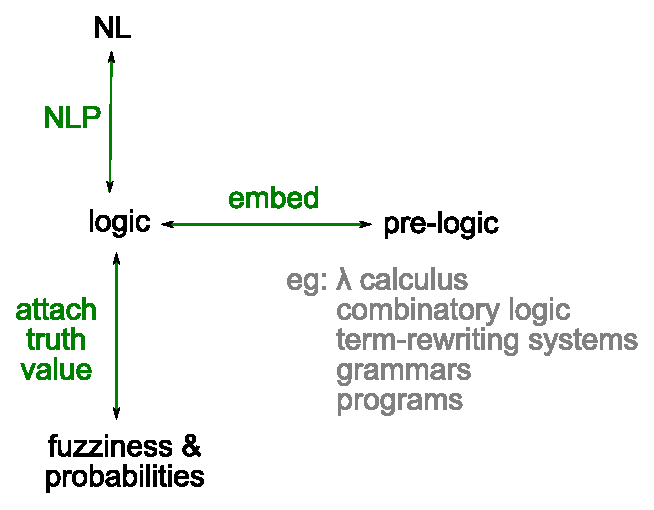
\includegraphics[scale=0.7]{prelogic.eps}
% \caption{Prelogic}
\end{figure}
NL should be translated into logic because logic is closer to NL than pre-logic.  What really distinguishes ``logic'' from pre-logic is the notion of \textbf{propositions}, which is a unit of meaning to which we can attach \textbf{truth values}.  A proposition such as \formula{male(john)} is a ``complete'' entity of meaning, as opposed to the predicate \formula{male} which is incomplete, or ``syncategorematic''\footnote{The term syncategorematic has several meanings, here I mean any component of a sentence that is not a proposition.}.  This distinction is important because fuzziness and probabilities should be assigned to the logic rather than pre-logic.

The problem with the above configuration is, if the pre-logic is fixed and the logic is allowed to be dynamically learned, then it may be difficult to work with such a dynamically changing logic, in particular to assign fuzzy-probabilistic truth values to it, or to translate NL to it.



\section{Uncertainty}

Reasoning under uncertainty is a vast and nightmarishly complex topic in AI.  Simon Parsons's book \citep*{Parsons2001} contains a very good survey of uncertain reasoning, but even that is not exhaustive.  We may look at the following taxonomy of ``ignorance'' proposed by \citep*{Bosc1997}:
\begin{figure}[H]
\centering
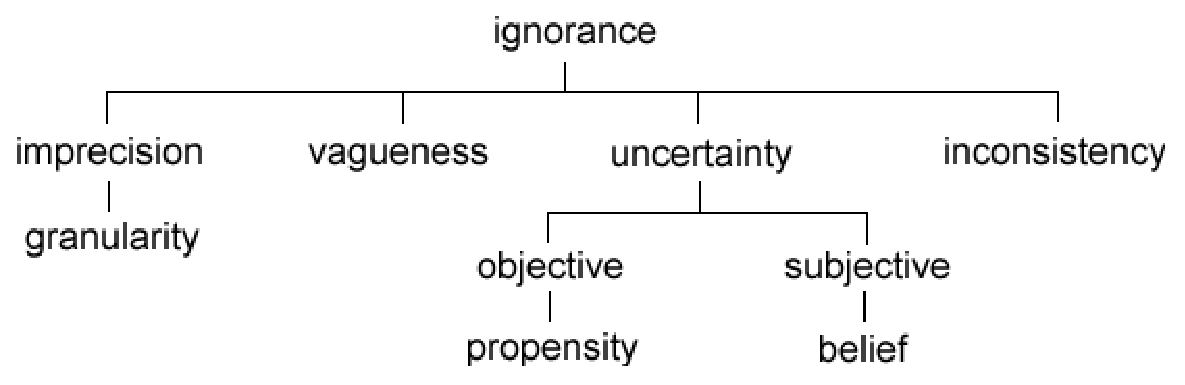
\includegraphics[scale=0.7]{IgnoranceTaxonomy.eps}
\caption{taxonomy of ignorance}
\end{figure}

At first blush, classical logic appears to be sufficient for AGI.  Some AGI designers prefer to use crisp logic as the base and plan to build $\mathcal{P}$ and $\mathcal{Z}$ upon crisp logic.  But this may be a sign of not facing problems and not having sufficient understanding of fuzzy-probabilistic logics.  To represent $\mathcal{P}$ and $\mathcal{Z}$ logic \textit{in} crisp logic is like writing an entire $\mathcal{P}$-$\mathcal{Z}$ inference engine in Prolog, complicated by the fact that the crisp logic would be somewhat different from Prolog and so may be even harder to program in.  Also, the ``truths'' known by the AGI will then be different from the truths as represented in the crisp logic --- the former would be ``floating'' above the latter;  This creates unnecessary indirectness.  I will give other reasons in \S\ref{sec:whyZ} and \ref{sec:whyP}.

\textbf{Why not include other uncertainty measures besides $\mathcal{P}$ and $\mathcal{Z}$?}

There are other theories of uncertainty, such as possibility, belief functions, and rough sets.  The reason I chose $\mathcal{P}$ and $\mathcal{Z}$ is because they are simple and best understood.  There has been attempts to create systems where the user can create a flexible number of uncertainty measures, but one problem of such systems has been pointed out in \citep*{Parsons2001}:  If we have 3 uncertainty measures, say ``cloud'', ``mist'', and ``fog'', there would be a need to provide mixed inference rules for ``cloud-mist'', ``cloud-fog'' etc, a total of $n^2$ possibilities.  I have worked out the combination of $\mathcal{B}$, $\mathcal{P}$ and $\mathcal{Z}$ and found that it involved considerable efforts.

\section{Modal logic}
\begin{flushright}
\emph{Modality, si! Modal logic, no!}\\
--- John McCarthy \citep*{McCarthy1997}
\end{flushright}

One argument for the use of modal logic arises from the following example:\\
\begin{tabular}{l l}
\hspace*{1cm} \textit{``John believes Superman is dead.''} & \formula{believe(john, dead(superman))}\\
\hspace*{1cm} \textit{``Superman is Clark Kent.''} & \formula{superman = clark-ken}\\
\hspace*{0.7cm} * \textit{``John believes Clark Kent is dead.''} & \formula{believe(john, dead(clark-ken))}
\end{tabular}\\
The problem is that John may not know that Superman is Clark Kent.

But another way to see it is that the problem arises from the use of the equality ``=''.  We may abandon \textbf{Leibniz extensionality}.  In other words, just because $A = B$ doesn't mean that everything about A automatically applies to B.

\underconst

\section{Shortcomings of the current logic}

1.  \textbf{Binary vs $\mathcal{P/Z}$.}  It may be desirable to have binary logic alongside $\mathcal{P/Z}$ logic.  $\mathcal{P/Z}$ reasoning is suitable for common-sense concepts, whereas binary reasoning is good for \textit{programmatic}
\footnote{Ie, binary logic makes programming easier}
or computational reasons.  However, one unsolved problem is that many common-sense concepts appear to be binary but are fuzzy upon close inspection (eg male/female, dead/alive).  The question is how to let binary and fuzzy concepts coexist in the same logic.

2.  \textbf{First-order vs Higher-order logic.}  Let us admit outright that FOL as a KR scheme is insufficient for common-sense reasoning and thus AGI.  But I also have the impression that second-order logic would be sufficient for most common-sense reasoning purposes.

With some tricks (such as reification, \S\ref{sec:reification}), FOL may be able to deal with second-order reasoning.

Another trick is that the FOL reasoner can ``escape'' to a meta-reasoner when higher-order constructs are needed.  This will be taken up on the chapter on meta-reasoning, \S\ref{ch:meta-reasoning}.

As a more satisfactory long-term solution, we are currently working on creating a $\mathcal{P(Z)C}$ HOL, see \S\ref{sec:HOL}.

%With P and Z, the AGI can express ideas such as:\\
%\hspace*{1cm} ``Mary is \underline{probably} \underline{fairly} tall.''

\section{$\mathcal{B}$: binary logic}
\label{sec:binary-logic}

My intuition is that common-sense reasoning involves mainly $\mathcal{B}$, followed by $\mathcal{Z}$, and $\mathcal{P}$ is relatively rare.

%Horn clauses:  P and Z rules can be expressed in Horn form only.  But it seems that we can use general resolution for B rules, no?  Or, perhaps I want to use something similar to Horn resolution for P and Z?

%Each rule will enable one inference step, so the logic is almost truth-functional.  The problem is the intermediate results... I only know how to do that in B form.  Maybe we can keep a set of disjunctions of truth values?

%In B logic the proof procedure keeps a current clause / or a line of clauses.  In Bayes net we have a query variable and the algorithm finds its P value.  Z logic may be similar to B logic because it's truth functional?

%Perhaps we can work out the general case of a query variable of any TV type?  If we draw a B rule that's easy.  If Z rule, then we have a few Z variables as goals.  They need Z rules to fulfill, but what if we have a B rule for one of the sub-goals?  Then we need to translate the B value to Z value.  We can only do that via P(Z).  So we have a P(Z) value as one of the subgoals.  This may cause the head of the rule to become P(Z) too.  It seems there is a tendency for all TVs to become P(Z).
%That will actually back-propagate along the proof sequence.

%Things may be even worse for a P rule.  The application of the rule requires other numbers.  

\section{Meta-reasoning}
\begin{flushright}
\emph{I think I think, therefore I think I am.}
\end{flushright}

The term ``meta-reasoning'' may refer to 2 things:\\
1. The ability to \textbf{reason about reasoning}, which is what this chapter is concerned with;\\
2. Scheduling reasoning tasks to achieve best results with limited computational resources (I have not thought about this problem yet).

An excellent survey of meta-reasoning in the \#1 sense is \citep*{Constantini2002}.

In the Tell-Learn loop, we see that we need a special predicate credible() to increase the probability of a statement via a side-effect.  But that may not be the only meta-reasoning move we can make.

Another example is the $B \leftrightarrow Z$ conversion of ``traitor'' and ``patriot'' (\S\ref{sec:PZ-meta-reasoning}).

\section{Higher order logic}
\label{sec:HOL}

The HOL formulation that I am most familiar with is \citep*{Lloyd2003}.  It uses \textbf{typed lambda calculus} to represent logical formulae.  This representation is specifically developed for use as a logic programming language (Escher) and for inductive learning.

Interestingly, Lloyd uses a form of algebraic logic that is similar to what I do with $\mathcal{P(Z)C}$ logic, ie, its statements are of the form $H = B$ where $H$ is the head and $B$ is the body.  In essence this is the Prolog / Horn tradition.

\{ TO-DO:  formulate a $\mathcal{P(Z)C}$ HOL \}

\label{sec:PZ-meta-reasoning}

One example of meta-reasoning pertinent to fuzziness is:\\
\hspace*{1cm} S1: ``You are either a patriot or a traitor.''\\
\hspace*{1cm} S2: ``No, I can be slightly patriotic or slightly traitorous.''

In S1 the predicates \textit{patriot} and \textit{traitor} have binary character.  In S2 they have fuzzy character.

\underconst

\include{vagueness}
\include{probabilities}
\include{confidence}
\include{inference}
\chapter{Pattern recognition}
\label{ch:pattern-recognition}
\minitoc

The diagram below is due to David Marr:
\begin{figure}[H]
\centering
\includegraphics[scale=0.7, bb=0 0 414 269]{Marr3DModel.PNG}
\end{figure}

A highly simplified example of pattern recognition is the visual recognition of a human body by a Prolog rule such as\footnote{
Note that these concepts refer to \textit{visual features} rather than ideas  (The abstract concept of a human can be recognized via a larger set of rules that includes the visual rules).  The visual features should also be related to each other by some spatial predicates, but we ignore them here.  The details of visual recognition is explained in \S\ref{ch:vision}.
}:\\
\hspace*{1cm} \code{human :- head, torso, arm1, arm2, leg1, leg2.}\\
and each body part can be further recognized by its components such as:\\
\hspace*{1cm} \code{arm1 :- upper-arm, forearm, hand, fingers.}

In general the mechanism for pattern recognition is \textbf{forward-chaining} because we start with the premises (sensory input) and we do not know the desired conclusions in advance.

\section{The theory-based theory}

Concept formation (or ``categorization'' in the cognitive science literature, \citep*{Murphy2002}, \citep*{Cohen2005}, \citep*{Margolis1999}, \citep*{Lakoff1987}) is the task of using machine learning to learn common-sense concepts (\citep*{Nakamura1993}, \citep*{Wrobel1994}).  \citep*{Wrobel1994} has summarized the following properties of human concepts:
\begin{compactenum}[1.]
\item concepts often have non-necessary features
\item disjunctive concepts (there may not be any features that are shared by all members of a concept)
\item relational information (seems to require first-order logic to represent)
\item some features are themselves concepts
\item typicality (people can often rank examples according to typicality, eg the most typical fruit is orange)
\item basic levels (people are more adapt at categorization at certain basic levels, eg naming an object ``chair'' rather than ``office chair'' or ``a piece of furniture'')
\item superordinate distance (eg ``chicken'' is rated more similar to ``animal'' than to ``bird'')
\item unclear cases (eg ``is tomato a fruit?'')
\item context-dependent effects
\item goal-dependent effects
\end{compactenum}

There are two major theories of categorization:  In the \textbf{Classical view} a concept is defined by a set of defining features which are individually necessary and sufficient.  This view has very few adherents now.  The other major theory is the \textbf{Exemplar view}, which classifies instances based on their similarity (eg a distance metric) to a set of existing exemplars.

In my opinion, also shared by \citep*{Murphy1985} and \citep*{Wrobel1994}, the most satisfactory solution (aka the \textbf{theory-based theory}) is to view categorization as an \textit{inference} process, where concept formation means constructing \textit{explanations} of why certain objects belong to a concept.

\section{Similarity}
\label{sec:similarity}

Similarity is an essential component of commonsense reasoning.  For example, if we are told that "the whale is like a fish except that it is a mammal" we could draw the conclusion that the whale can swim (because fishes usually can swim) \footnote{But we would not conclude that the whale lays eggs because mammals don't lay eggs and we know that the whale \emph{is} a mammal, but it is only similar to a fish, and "is" is stronger than "similar to".}.
  
The similarity measure may also help in associative recall (\S\ref{sec:associative-memory}).

Similarity can be defined as an equivalent relation $\approx$, analogous to the equality relation $=$.  For example we can write\\
\tab $\mbox{whale} \approx \mbox{fish}$.

Recall that equality ($=$) is defined by \textbf{Leibniz's axiom of extensionality} -- which states that 2 entities are the same if every property of one is also a property of the other.  In type theory it can be stated as:
\begin{equation}
\forall x [f x = g x] \Rightarrow f = g
\label{eqn:Leibniz-extensionality}
\end{equation}
with $x : \beta$ and $f, g : \beta \rightarrow \alpha $.  This definition of $=$ is given by Church's type theory in 1940.  It defines equality for any function / predicate / proposition.

The similarity $\approx$ can be regarded as the probabilistic version of $=$.  We can simply replace the $\forall$ quantification in (\ref{eqn:Leibniz-extensionality}) with the probabilistic quantification $\#$ (\S\ref{sec:probabilistic-quantifier}), as in:
\begin{equation}
\# x [f x = g x] \Rightarrow f \approx g.
\label{eqn:probabilistic-extensionality}
\end{equation}

But there is one problem.  In the whale $\approx$ fish example, the similarity is there not because the whale and fish predicates can apply to many common members (in fact, the 2 classes have no overlaps);  but because there are \textit{other} predicates that apply to both of them as objects.  For example:

\tab \tab \tab
\begin{tabular}{l|l}
has-fins(whale)        & has-fins(fish)\\
lives-in(whale, water) & lives-in(fish, water)\\
vertebrate(whale)      & vertebrate(fish)\\
\end{tabular}

How to capture this?  The solution is to ``turn around'' Leibnez's definition thusly:
\begin{eqnarray}
\mbox{(Leibnez)}                 & \forall z. [x z = y z] \Rightarrow& x = y \\
\mbox{(inverted Leibnez)}     & \forall z. [z x = z y] \Rightarrow& x = y
\label{eqn:inverted-extensionality}
\end{eqnarray}
where I have renamed the variables to stress the symmetry.  And the probabilistic form is:
\begin{equation}
\# z [z x = z y]  \Rightarrow x \approx y.
\end{equation}
Notice that if we use higher-order logic, $z$ can be unified with n-ary predicates with other arguments, eg
 $$z(x) = \mbox{lives-in}(x, \mbox{water})$$
so this is a very powerful way that can express all forms of similarities.

\{ To-do:  I need to develop the above theory further.  Milner's Context Lemma in domain theory seems to have some semblance to what we're doing here.  Milner's Lemma states the equivalence of 2 orderings, $<_{\sigma}$ and $\sqsubset$.  They are defined by:
\begin{eqnarray}
M \sqsubset N        \quad     & \mbox{iff} &    \quad \forall z \in \setN. \; M \Downarrow z \Rightarrow N \Downarrow z \\
M <_{\sigma} N    \quad     & \mbox{iff} &    \quad \forall Z \in \mbox{programs.} \; Z(M) \sqsubset Z(N)
\end{eqnarray}
where $M \Downarrow z$ means $M$ evaluates to $z$.  The situation resembles Leibniz's definition and its ``inverted form''.
\}

We'd be interested in measuring similarities between entities with certain structures.  This has been considered, eg in \citep*{Schmid2003}, chapters 10-12, in an ILP setting.  A famous example is the similarity between the solar system and the atom:  the important point is that both systems have bodies revolving around a central body, but it does not matter what their size, mass, and temperature, etc, are.

\{ The text that follows is outdated material... \}
\underconst

What we seek is a correspondence between 2 structured entities, and to quantitatively measure the strength of such a correspondence.  Perhaps we can count the number of relations common to both entities.

\subsection{Motivating examples}

(A) ``Marmite is similar to Vegemite''\\
\hspace*{1cm} \begin{tabular}{l|l}
salty(marmite)                   & salty(vegemite)\\
dark-brown(marmite)              & dark-brown(vegemite)\\
yeast-extract(marmite)           & yeast-extract(vegemite)\\
rich-in(marmite, vitamin B)      & rich-in(vegemite, vitamin B)\\
sub-string(name(marmite),"mite") & sub-string(name(vegemite),"mite")\\
popular-in(england)              & popular-in(australia)
\end{tabular}

So I propose that the similarity between 2 objects can be calculated by considering all predicates that apply to both objects and obtaining the ratio between the number of identical and different predicates:
\begin{equation}
\mbox{similarity } \; \psi = \frac{N^{=}}{N^{=} + N^{\neq}}
\end{equation}

\{ TO-DO:  If the predicates have complex structure, we need to (recursively) compare the other arguments, and if the latter are different, adjust for their differences. \}

The above calculation can also be weighted by \textbf{information utility}, yielding the \textbf{subjective similarity} measure.

NOTE:  (B) is a bad example and should be replaced by something else.\\
(B) ``Lincoln is similar to Kennedy''
\footnote{In this example I have used my own knowledge representation scheme Geniform.  The example is based on a series of uncanny coincidences between the Lincoln and Kennedy assassinations that are often cited in trivia books.}
\\
\hspace*{1cm} \begin{tabular}{l|l}
elected-to-congress(lincoln, 1846)        & elected-to-congress(kennedy, 1946)\\
elected-president(lincoln, 1860)          & elected-president(kennedy, 1960)\\
succeeded-by(lincoln, vice-president$_1$) & succeeded-by(kennedy, vice-president$_2$)\\
\hspace*{1cm} name(vice-president$_1$, "johnson") &
\hspace*{1cm} name(vice-president$_2$, "johnson")\\
\hspace*{1cm} born(vice-president$_1$, 1808) &
\hspace*{1cm} born(vice-president$_2$, 1908)\\
assassinated$_1$(lincoln, friday)         & assassinated$_2$(kennedy, friday)\\
in(assassinated$_1$, theater)             & in(assassinated$_2$, car)\\
name(theater, "ford")                     & made(car, "ford")\\
with$_1$(wife(lincoln), lincoln)          & with$_2$(wife(kennedy), kennedy)\\
\hspace*{1cm} during(with$_1$, assassination$_1$) &
\hspace*{1cm} during(with$_2$, assassination$_2$)\\
\end{tabular}

Additionally:\\
\hspace*{1cm} name(car, "Lincoln")\\
\hspace*{1cm} has(kennedy, secretary), name(secretary, "Lincoln")

The additional facts do not increase the similarity, but they do make the 2 cases seem more ``connected''.

\underconst

(C) Some quantitative examples:\\
\hspace*{1cm} \begin{tabular}{|l|l|l|}
\hline
\textbf{the thing} & \textbf{approximated as} & \textbf{reason}\\
\hline
orange T-shirt     & red T-shirt      & proximity in color space\\
7 people           & several people   & $\mathcal{Z}$\\
6'5 tall           & very tall        & $\mathcal{Z}$\\
(John lies on several occasions) & John often lies & $\mathcal{P}$\\
Stewart Shapiro    & Stuart Shapiro   & string edit distance\\
\hline
\end{tabular}

These examples can be represented and approximated by $\mathcal{P/Z}$ values (eg with fuzzy pattern recognition).

%orange(t-shirt) -> red(t-shirt)
%7*people -> several*people
%height(john,6.5) -> tall(john)
%(multiple facts) -> lies1(john), often(lies1)
%"Stewart Shapiro" -> "Stuart Shapiro"

(D) Some qualitative examples:\\
\hspace*{1cm} John is humorous $\approx$ John is witty\\
\hspace*{1cm} junk food, smoking and drinking $\approx$ unhealthy lifestyle\\
\hspace*{1cm} theft $\approx$ burglary\\
\hspace*{1cm} (complex scene) $\approx$ a fighting in a bar


\include{belief-revision}
\include{induction}
\chapter{Natural language}
\label{ch:natural-language}
\begin{flushright}
\emph{The fish trap exists because of the fish; once you've gotten the fish,\\
you can forget the trap. The rabbit snare exists because of the rabbit;\\
once you've gotten the rabbit, you can forget the snare.\\
Language exists because of meaning; once you've gotten the meaning,\\
you can forget language.}\\ --- Zhuangzi (4th Century BC)
\end{flushright}
\minitoc

\section{Natural language is not essential to AGI}

Our approach is to define a logic that can faithfully render arbitrary natural-language texts.  We call such a logical form Geniform.  The translation of NL to Geniform can itself be encoded as logical rules, thus the parsing of NL can be achieved via logical inference (as forward-chaining in a bottom-up manner).  And since logical inference is reversible, the generation of NL will also come as free.

All the irregularities of NL will be taken care of via machine learning.

\subsection{Multiplicity of knowledge representation schemes}

This is how I think of the issue of knowledge representation:\\
\begin{figure}[H]
\centering
\includegraphics[scale=0.7]{KR-functors.png}
% \caption{KR functors}
\end{figure}

There are various KR schemes.  For example, in NL, there are various grammar formulations\\
$F$ may be Phrase Structure Grammar.\\
$G$ may be Fluid Construction Grammar.\\
$H$ may be Categorial Grammar.\\
$J$ may be Geniform (a simple grammar I designed for Genifer)\\
$K$ may be Genifer's machine-learned grammar (which may be stochastic and inscrutable to humans)

And then there would be transformations ($\eta, \epsilon, ...$) between the grammatical formalisms.

The problem is whether we can mix multiple KR schemes like $F$ and $G$.  The commonsense KB would be different under either $F$ or $G$, and the entire KB needs to be transformed by some $\eta$.

If we use $F, G, H,...$ at the same time, confusion may arise during machine learning and reasoning.

Perhaps, if we make Genifer be aware of transformations like $\eta, \epsilon, ...$ then maybe it can deal with multiple KR schemes at the same time?  Therefore we maybe don't need to choose or commit to any particular KR scheme at this stage...  in other words, any would be fine.

\subsection{Background: unification-based grammars}

The family of unification-based grammars includes LFG (Lexical Functional Grammar), HPSG (Head-Driven Phrase Structure Grammar), and PATR grammar.  The unification algorithm used in unification-based grammar is the same as the unification algorithm used in logic.  This is further evidence that the brain employs abstract symbolic processing similar to formal logic.

\subsection{Background: cognitive linguistics}

Our approach is closer to ``formal semantics''.  Many authors, most famously Richard Montague, have argued that natural languages are formal languages.  Some have also advocated the use of natural language as knowledge representation in AI.  Thus the line between formal and natural languages is blurred.

\todo{How may cognitive linguistics affect natural language processing in Genifer?}

\section{Abduction as interpretation}
\label{sec:abduction-as-interpretation}

\subsection{A detailed example}

The general sequence is:\\
\hspace*{1cm} tokenization $\rightarrow$ POS-tagging $\rightarrow$ syntax parsing $\rightarrow$ semantic parsing\\
which should be familiar to everyone with experience in NL processing.

I will explain the details using a simple example:\\
\hspace*{1cm} ``I love Mary''

The crucial thing is that we represent everything in a logic-based framework. First we represent the sentence as "raw data" (ignoring tenses to simplify matters):\\
\hspace*{1cm} $\mbox{sentence}(e_0)$\\
\hspace*{1cm} $\mbox{lexeme-I}(e_1)$\\
\hspace*{1cm} $\mbox{lexeme-love}(e_2)$\\
\hspace*{1cm} $\mbox{lexeme-Mary}(e_3)$\\
\hspace*{1cm} $\mbox{begins-with}(e_0, e_1)$\\
\hspace*{1cm} $\mbox{follows}(e_2, e_1)$\\
\hspace*{1cm} $\mbox{follows}(e_3, e_2)$\\
where:\\
\hspace*{1cm} the $e_i$'s are \textbf{entities} (logical constants).\\
\hspace*{1cm} the entities $e_1$, $e_2$, and $e_3$ are words.\\
\hspace*{1cm} follows() means a word follows another word in a sentence.

Up to now, all we have is a sentence as raw text (without meanings).  The next step is to recognize parts of speech (nouns, verbs, adjectives, etc). We can use logical rules to do this.

An example logical rule is:\\
\hspace*{1cm} $\mbox{lexeme-Mary}(X) \rightarrow \exists e \; \mbox{parse-as}(e, X) \wedge \mbox{noun}(e)$\\
which simply means that the word "Mary" is a noun. X is a variable (implicitly universally quantified). $e$ is a new entity, which instantiates to $e_4$ when the rule is applied.

We can also use logical rules to parse syntax. We can perform ``VP $\leftarrow verb + noun$'' with this rule\footnote{We need this special rule:\\
\hspace*{1cm} $\mbox{follows}(X_1, X_2) \wedge \mbox{parse-as}(X_1, X_3) \wedge \mbox{parse-as}(X_2, X_4) \rightarrow \mbox{follows2}(X_3, X_4)$ }:\\
\hspace*{1cm} $\mbox{verb}(X_1) \wedge \mbox{noun}(X_2) \wedge \mbox{follows2}(X_2, X_1) \rightarrow \exists e \; \mbox{parse-as}(e, X_1, X_2) \wedge vp(e)$\\
which creates a new entity $e_5$ which is a VP.

Assume that eventually we have a parse of the sentence S, $e_6$. Notice that up to now, it's all syntax parsing.

Next we perform semantic parsing.  The key is to generate partial meanings for phrases, such as the verb phrase ``loves Mary''.

\textbf{Lambda operator.}  In formal semantics, it is customary to use the $\lambda$ operator to represent the meaning of phrases.  The reason is that first-order logic do not have the expressive power to represent such phrases.  For example, the VP ``loves Mary'' denotes ``somebody's loving Mary'', which may be represented as $love(\_ \,,mary)$; but that is not a well-formed formula in FOL.  Instead we can represent it using the $\lambda$ expression $\lambda x \; love(x,mary)$.

\textbf{Composition of concepts.}  (For details see \S\ref{sec:composition})  Under this method, all phrases are represented by compositions.  For example, the VP ``loves Mary'' can be represented by $app(loves,mary)$, or in short form $mary \circ loves$.  This composite is a \textit{first-order object}, ie, a first-class citizen in the logic which can be further manipulated or modified, eg, when we compose it with $john$, we get $((mary \circ loves) \circ john)$ which is equivalent to the FOL statement $loves(john,mary)$.

I think this method is superior to $\lambda$ because the meanings of phrases can be represented by first-order objects.  It also makes semantic parsing very intuitive.

% \todo{Revise this example with the newly improved Geniform.}

\todo{Explain semantic parsing with examples.}

%A semantic rule is similar to a syntactic one:\\
%\hspace*{1cm} $\mbox{lexeme-love}(X) rightarrow \exists e \; \mbox{parse-as}(e, X) \wedge \mbox{verb}(e) \wedge \mbox{means}(e, \mbox{concept-love})$\\
%
%\hspace*{1cm} $\mbox{verb}(X_1) \wedge \mbox{np}(X_2) \wedge \mbox{follows2}(X_2, X_1) \wedge \mbox{means}(X_1, Y_1) \wedge \mbox{means}(X_2, Y_2)$\\
%\hspace*{1cm} $rightarrow \exists e \; \mbox{parse-as}(e, X_1, X_2) \wedge vp(e) \wedge \mbox{means}(e, comp(Y_1,Y_2))$\\
%
%For example, we can augment the syntactic rule\\
%\hspace*{1cm} $\mbox{VP} \leftarrow \mbox{verb}, \mbox{NP} $\\
%with\\
%\hspace*{1cm} $\mbox{VP}(\mbox{comp}(Sem_1,Sem_2)) \leftarrow \mbox{verb}(Sem_1), \mbox{NP}(Sem_2)$\\
%where the $Sem$'s are variables containing the ``semantics'' of phrases.\\
%\hspace*{1cm} $\mbox{S} \leftarrow \mbox{NP}, \mbox{VP} $\\
%\hspace*{1cm} $\mbox{S}(Predicate) \leftarrow \mbox{NP}(Subject), \mbox{VP}(Subject * Predicate) $\\
%\hspace*{1cm} $\mbox{VP}(X) rightarrow \mbox{com}(\mbox{loves},\mbox{mary})$\\
%which creates a new entity $e_7$ with the meaning of "love".\\
%\hspace*{1cm} $\mbox{lexeme-love}(X_1) rightarrow \exists e \; \mbox{concept}(e) \wedge \mbox{means}(e, \mbox{concept-love})$\\
%
%The final step of semantic parsing uses a special trick,  ``de-reification'' (\S\ref{sec:reification}):\\
%\hspace*{1cm} (assume that $e_{8}, e_{9}$ denote the persons John and Mary)\\
%\hspace*{1cm} $\mbox{de-reify}(\mbox{concept-love}, e_{8}, e_{9})$\\
%which generates the logical statement:\\
%\hspace*{1cm} $\mbox{loves}_1(e_{8},e_{9})$\\
%
%Finally we have:\\
%\hspace*{1cm} $\mbox{means}(e_0, \mbox{loves}_1)$

\section{Comprehensive grammatical categories of English}

Here are some NL grammatical categories (intended to cover as broadly as possible) and typical examples in English.  Designers of NL interfaces can supply translations to these examples.  [The contents in this section and all the examples are taken directly from the book "English Grammar" by Peter Collins, 1998, Addison Wesley.  \textbf{NOTE:  This may be a copyright infringement but I have contacted the author without getting his reply.}]  This page is intended to provide a simple comparison of NL interfaces, not meant to be a standard grammar for AGI purposes.

\titleformat{\subsection}[hang]{\sffamily\bfseries\large\color{blue}}{(\Alph{subsection}) \hspace{5pt}}{0pt}{}

\setcounter{subsubsection}{1}
\renewcommand{\subsubsection}[1]{\sffamily{\bfseries{\color{blue}{ \stepcounter{subsubsection} (\Alph{subsection}.\arabic{subsubsection}) \hspace{5pt}#1}}}}

\newcounter{subsubsubsection}[subsubsection]
\newcommand{\subsubsubsection}[1]{\stepcounter{subsubsubsection} \sffamily{\bfseries{\color{blue}{ (\Alph{subsection}.\arabic{subsubsection}.\arabic{subsubsubsection}) \hspace{5pt}#1}}}}

\subsection{Nouns}

\subsubsection{Common nouns}

eg "chair", "chairs"

eg "importance"

\subsubsection{Proper nouns}

eg "Australia"

eg "The Isle of Man"

\subsubsection{Pronouns}

eg "he"

eg "\textbf{our} chair" (possessive, as determiner)

eg "theirs"

eg "each other", "one another" (reciprocal pronouns)

eg "this", "that" (demonstrative pronouns)

eg "who", "whom", "whatever" (interrogative and relative pronouns)

eg "some", "both", "any", "each", "none", "nobody" (indefinite pronouns)

\subsection{Verbs}

\subsubsection{Main verbs}

eg "kick", "grow"

eg "to kick", "kicked", "kicking", "kicks" (tenses and other inflections)

\subsubsection{Auxiliary verbs}

eg "can", "have", "haven't"

eg "She \textbf{is} dancing the lambada."

eg "He \textbf{has} driven for 4 hours."

\subsubsection{Operators}

eg "they \textbf{will} try their best", "Sam \textbf{won't} play chess"

\subsection{Adjectives}

\subsubsection{Attributive (modifies a head noun)}

eg "the \textbf{loud} bell"

\subsubsection{Predicative}

eg "the bell was \textbf{loud}"

\subsubsection{Gradation}

eg "\textbf{very} loud", "\textbf{a bit} loud"

\subsubsection{Comparison}

eg "louder", "loudest"

\subsection{Adverbs}

eg "The policeman acted \textbf{decisively}"

eg "He is a \textbf{somewhat} shy young man"

eg "\textbf{Actually}, many of the lifeboats have been removed"

eg "Patrick has lost 2 games, \textbf{however} he could still win"

eg "more surprisingly", "most surprisingly"

\subsection{Determinatives}

\subsubsection{Articles}

eg "the", "a", "an"

\subsubsection{Demonstratives}

eg "this", "that", "those"

\subsubsection{Interrogatives}

eg "which", "what"

\subsubsection{Cardinal numerals}

eg "one", "two"

\subsubsection{Quantifiers}

eg "both", "all", "every", "any", "no", "much", "less"

\subsubsection{Prepositions}

\subsubsubsection{Time}


eg "\textbf{after} our match", "\textbf{during} the exam"

\subsubsubsection{Place}


eg "\textbf{in} the kitchen", "\textbf{against} the wall"

\subsubsubsection{Manner}


eg "\textbf{with} ease"

\subsubsubsection{Agency}


eg "\textbf{by} the mechanic"

\subsubsubsection{Recipience}


eg "\textbf{to} a friend"

\subsubsection{Subordinates}

\subsubsubsection{Time}


eg "\textbf{until} it rains", "\textbf{as} she spoke"

\subsubsubsection{Condition}


eg "\textbf{if} we win Lotto", "\textbf{unless} a catastrophe occurs"

\subsubsubsection{Concession}


eg "\textbf{although} she likes coffee", "\textbf{while} it was undoubtedly entertaining"

\subsubsubsection{Contrast}


eg "\textbf{whereas} Japan is a creditor nation"

\subsubsubsection{Exception}


eg "\textbf{except} he didn't have the strength"

\subsubsubsection{Reason}


eg "\textbf{because} the bus broke down"

\subsubsubsection{Comparison}


eg "you ate more peanuts \textbf{than} I did"

\subsubsection{Coordinators}

eg "Peter went to Paris \textbf{but} his family stayed home"

eg "Barbie was wearing a new bracelet \textbf{and} a diamond ring"

eg "Should we come before \textbf{or} after lunch?"

eg "\textbf{Both} Bill \textbf{and} his wife deny the allegations"

eg "She \textbf{neither} hates him \textbf{nor} loves him"

eg "It's \textbf{not} for you \textbf{but} for me"

\subsection{Phrases}

\subsubsection{Noun phrase (NP)}

eg "large birds with sharp claws"

eg "writers of science fiction, who are here for a conference"

\subsubsection{Verb phrase (VP)}

eg "[Lisa] \textbf{trains} 3 times a week"

eg "There I \textbf{am}, minding my own business, when this tall blonde \textbf{walks} up and \textbf{asks} me for a cigarette"

eg "Ken said, 'I \textbf{have} enough money' "

eg "[If I] \textbf{could} have my life over again, [I] \textbf{would} not change anything"

eg "[They should] \textbf{have reached} the peak by now"

eg "[Ken] \textbf{is} building a new house"

eg "[Many footballers] \textbf{get} injured"

\subsubsection{Adjective phrase (AdjP)}

eg "too rebellious", "quite surprisingly intelligent", "very slow"

eg "slower than a wet week", "large for a goldfish"

eg "fiercer than I expected"

eg "sorry that he hurt her feelings" (noun clause)

eg "aware of the consequences" (of-PP)

\subsubsection{Adverb phrase (AdvP)}

eg "very quickly", "most reluctantly"

eg "more defiantly than they had predicted"

\subsubsection{Prepositional phrase (PP)}

eg "\textbf{in} the water"

eg "\textbf{with} a spoon"

eg "[way] \textbf{below} standard", "[just] \textbf{before} the start"

eg "Scott arrived \textit{in} \textbf{a limousine} \textit{with} \textbf{his girlfriend}"

\subsubsection{Genitive phrase (GP)}

eg "\textit{The princess's} popularity was greater than \textit{her husband's}"

\subsection{Clauses}

\subsubsection{Object vs predicative complements}

eg "Mary contacted \textbf{a police officer}" (object)

eg "Mary was \textbf{a police officer}" (predicative, "was"=copula)

\subsubsection{Subjective and objective predicatives}

eg "Indira was \textbf{generous}" (subjective)

eg "We considered Indira \textbf{generous}" (objective)

\subsubsection{Patterns of complementation}

\subsubsubsection{intransive (S P)}

eg "Sue \textbf{stumbled}"

\subsubsubsection{monotransitive (S P Od)}

eg "Sue \textbf{sipped a martini}"

\subsubsubsection{Copulative (S P PCs)}

eg "Sue \textbf{seems drunk}"

\subsubsubsection{Ditransitive (S P Oi Od)}

eg "Sue \textbf{offered her guests a martini}"

\subsubsubsection{Complex-transitive (S P Od PCo)}

eg "Sue \textbf{made them drunk}"

\subsubsection{Other complements}

\subsubsubsection{PP-complements of prepositional verbs}

eg "They have decided \textbf{on a short vacation}"

eg "He approves entirely \textbf{of your decision}"

eg "Geoff protected his little brother \textbf{from the bullies}"

eg "She blames all their problems \textbf{on his incompetence}"

\subsubsubsection{Adverbs as complement of phrasal verbs}

eg "Vera cried \textbf{out}"

eg "We give \textbf{up}"

eg "The umpires have called \textbf{off} the match"

eg "Please take the garbage \textbf{out}"

eg "We have come \textbf{up} \textbf{with an alternative plan}"

\subsubsubsection{Non-finite complements of 'catenative' verbs}

eg "I \textbf{plan} to \textbf{keep} applying for jobs"

eg "You should \textbf{stop} \textbf{trying} to \textbf{get} invited"

\subsubsection{Adjuncts}

AdvP: eg "very carefully", "sometimes", "moreover"

PP: eg "over the road", "with a torch"

Subordinate clause:  eg "because it is raining" "after the music stopped"

NP: eg "next Easter" "this Friday"

types:

Time:  eg "at Easter" "in 2 week's time"

Frequency:  eg "each Friday" "on the hour"

Place: eg "in Bandung" "on the summit"

Purpose: eg "in order to test the hypothesis" "for a break"

Reason: eg "because he is shy" "on the grounds of sanity"

Condition: eg "if you agree" "unless it is convenient"

Manner: eg "more politely" "with a spade"

Degree: eg "in my opinion" "to be fair" "unfortunately"

Connective: eg "consequently" "in other words" "however"

\subsubsection{Mood}

\subsubsubsection{Declarative mood}

eg "He is serious"

\subsubsubsection{Interrogative mood}

eg "Is he serious?"

eg "Anastasia has sent another e-mail, hasn't she?"

eg "Whose T-shirt is that?"

eg "Who can help me?"

eg "Where are my keys?"

\subsubsubsection{Imperative mood}

eg "Be serious"

eg "Give me some more money"

eg "Don't forget to write"

eg "Let's apply for a loan"

\subsubsubsection{Exclamative mood}

eg "How serious he is!"

eg "How many times have I asked you!"

\subsubsection{Negation}

clausal negation:  eg "Courtney is \textbf{not} reading"\\
                   eg "We have heard \textbf{nothing}"\\
                   eg "\textbf{Nobody} likes a loser"\\
                   eg "We \textbf{barely} made it"\\
                   eg "They \textbf{seldom} celebrate birthdays"

sub-clausal negation:  eg "Karen is very \textbf{unfriendly}"\\
                      eg "The ambulance arrived \textbf{not long ago}"

\subsection{Subordination and coordination}

\subsubsection{Subordinative clause (complex sentence)}

eg "I know \textbf{that Ella lives in Sydney}"

eg "He knows a woman \textbf{who lives in Sydney}"

eg "He asked \textbf{whether anyone had submitted a nomination}"

\subsubsubsection{Adverbial clauses}

time:  eg "Angelica will not agree to it \textbf{until his attitude improves}"

place:  eg "he goes \textbf{wherever his fancy takes him}"

etc

\subsubsubsection{Relative clauses}

eg "Is that the boy who you were referring to?"

eg "I remember the days when none of us had a care in the world"

eg "I know who is replacing you"

eg "Whatever is now developing can only cause harm"

\subsubsubsection{Comparative clauses}

eg "He performed worse than you did"

eg "Tim has won a larger grant than I have"

eg "She is as tall as we had anticipated"

\subsubsubsection{Non-finite clauses}

infinitival: eg "Sharon wants to \textbf{apply next year}"

present-participle: eg "Sharon favors \textbf{applying next year}"

past-participle: eg "Sharon has her application \textbf{lodged already}"

past-participle: eg "Anyone \textbf{caught smoking here} can be prosecuted"

\subsubsubsection{Verbless clauses}

eg "\textbf{If in doubt} consult your solicitor"

eg "He visits his parents \textbf{whenever possible}"

eg "\textbf{With Claudia in charge} we should be able to regain control"

\subsubsection{Coordinated clause (compound sentence)}

eg "Ella lives in Sydney, but she was born in China"

eg "Daphne like classical music \textbf{but} her husband prefers jazz"

\subsection{Information packaging}

\subsubsection{Topic}

eg "Leonardo da Vinci painted the Mona Lisa"\\
vs "The Mona Lisa was painted by Leonardo da Vinci"

\subsubsection{Focus}

eg "The judges gave near maximum points to Lipinsky"\\
vs "The judges gave Lipinsky near maximum points"

\subsubsection{Weight (more weight near end of sentence)}

eg "It surprised us that an Australian skier could win a medal in the slalom event at the Nagano Olympics"\\
vs "That an Australian skier could win a medal in the slalom event at the 
Nagano Olympics surprised us"

\subsubsection{Voice}

active: eg "Sergeant Rogerson arrested the thief"\\
passive: eg "The thief was arrested by Sergeant Rogerson"

eg "Each specimen was carefully dissected"

\subsubsection{Cleft sentences}

eg\\
"Whitlam recalled the remaining troops from vietnam"\\
"It was Whitlam who recalled the remaining troops from Vietnam"\\
"It was the remaining troops that Whitlam recalled from vietnam"\\
"It was from Vietnam that Whitlam recalled the remaining troops"

eg\\
"Salt air can cause rust"\\
"What can cause rust is salt air"\\
"Salt air is what can cause rust"

\subsubsection{Extraposition}

eg "It is a pity that CDs are so expensive"

\subsubsection{Existential sentences}

eg "There is a fly in my soup"

eg "There's been another oil spill"

eg "There's a present for you"

eg "There followed a new round of toasts"

\subsubsection{Reordering}

\subsubsubsection{Subject-complement reversal}

eg "Tom is the short one"\\
$\Longrightarrow$ "The short one is Tom"

\subsubsubsection{Topicalization}

eg "He rejects totally the corruption charge"\\
$\Longrightarrow$  "The corruption charge he rejects totally"

eg "It rained for most of the day last Saturday"\\
$\Longrightarrow$  "Last Saturday it rained for most of the day"

\subsubsubsection{Locative inversion}

eg "Another F15 appeared from behind the clouds"\\
$\Longrightarrow$  "From behind the clouds appeared another F15"

\subsubsubsection{Dislocation}

eg "Dr Davidson's never available on Wednesdays"\\
$\Longrightarrow$  "(As for) Dr Davidson, he's never available on Wednesdays"

\subsubsubsection{Dative movement}

eg "Steve gave a red rose to his girlfriend"\\
$\Longrightarrow$  "Steve gave his girlfriend a red rose"

\subsubsubsection{Extraposition from NP}

eg "A position for someone with programming expertise is available"\\
$\Longrightarrow$  "A position is available for someone with programming expertise"

\subsubsection{Some grammatical devices}

\subsubsubsection{Co-reference}

eg "Your sister rang yesterday. \textbf{She} asked if you could call her back."

eg "It is inadvisable to visit Jakarta at present.  Civil unrest has broken out \textbf{there}."

\subsubsubsection{Ellipsis}

eg "Come whenever you can [come]"

eg "Somebody should help dad.  I'll ask Barry to [help dad]."

\subsubsubsection{Substitution}

eg "I have 2 spare tickets for the concert.  Would you like \textbf{one}?"

eg "She achieved less this year than she \textbf{did} last year."

eg "I'll collect the kids after school if you don't get the opportunity to \textbf{do so}."

\titleformat{\subsection}[hang]{\sffamily\bfseries\large\color{blue}}{\thesubsection \hspace{5pt}}{0pt}{}

\renewcommand{\subsubsection}[1]{\sffamily{\bfseries{\color{blue}{ \stepcounter{subsubsection} #1}}}}

\section{Geniform -- a logical form for natural language}
\label{sec:geniform}

% Rus proposed a popular logical form for rendering natural language, which is of reference value.  Geniform has made several significant improvements over it.

The Geniform logical form is special in that it can represent all natural-language grammatical categories elegantly.  To illustrate this, consider:\\
\hspace*{1cm} ``John loves Mary''\\
which is rendered in predicate logic as:\\
\hspace*{1cm} \formula{loves(john, mary)}\\
(ignoring tense).  But what if we want to say:\\
\hspace*{1cm} ``\textit{Loving Mary} is foolish'' ?\\
The verb phrase ``loving Mary'' is a grammatical unit that has a specific meaning but it cannot be represented in predicate logic.  In computational linguistics we usually use the \textbf{$\lambda$-abstraction} to represent it:\\
\hspace*{1cm} \formula{$\lambda$x.loves(x, mary)}\\
but as you can see, this form is not very human-readable.

The innovation of Geniform is to replace $\lambda$-abstractions with combinators \footnote{As in combinatory logic, a formalism equivalent in expressive power as $\lambda$ calculus.}.  For example,\\
\hspace*{1cm} \formula{loves(x, y)}\\
is represented in \textbf{curried form}\footnote{In honor of the logician Haskell B Curry.}:\\
\hspace*{1cm} \formula{\textbf{loves} = $\lambda$y($\lambda$x.loves(x,y))}\\
so that \formula{\textbf{loves}} is equivalent to the original predicate but it takes its arguments one at a time.

Now we can represent elements like:\\
\hspace*{1cm} ``John loves ....'' as \formula{(\textbf{loves} john)} and\\
\hspace*{1cm} ``.... loves Mary'' as \formula{(\textbf{C loves} mary)}\\
where \formula{\textbf{C}} is a combinator with the property \formula{\textbf{C}XYZ = \textbf{C}XZY}.

( TO-DO:  With the use of combinators, our logic is no longer a first-order logic, but some kind of higher-order logic.  Indeed, the naive form of this logic will be affected by problems like the Liar's Paradox. )

Anyway, Geniform can now express most NL categories.  For example:\\
\hspace*{1cm} chair $\Longrightarrow$ \formula{chair(chair$_1$)}\\
\hspace*{1cm} wooden chair $\Longrightarrow$ \formula{chair(chair$_1$), wooden(chair$_1$)}\\
\hspace*{1cm} a chair $\Longrightarrow$ \formula{chair(chair$_1$), a(chair$_1$)}\\
\hspace*{1cm} 3 chairs $\Longrightarrow$ \formula{chair(chair$_1$), 3(chair$_1$)}\\
\hspace*{1cm} 3 wooden chairs $\Longrightarrow$ \formula{chair(chair$_1$), 3(chair$_1$), wooden(chair$_1$)}\\
\hspace*{1cm} any chair $\Longrightarrow$ \formula{chair(chair$_1$), any(chair$_1$)}\\
\hspace*{1cm} no chair $\Longrightarrow$ \formula{chair(chair$_1$), no(chair$_1$)}\\
where \formula{chair$_1$} is an \textbf{instantiation} of the concept ``chair'', ie, a new constant \formula{chair$_1$} is created and ``\formula{chair(chair$_1$)}'' is asserted.  Notice that \formula{chair$_1$} does not denote \textit{one} chair; it is just an instantiation of the abstract concept of ``chair''; additional predicates are needed to specify it.  For example, the application of \formula{a()} or \formula{the()} specifies that \formula{chair$_1$} is singular, and the application of \formula{3()} specifies that \formula{chair$_1$} numbers 3.  It may stretch your understanding a bit to think of ``any chair'' and ``no chair'' as instances of ``chair'', but I think the idea is sound.

Now let's add some syntactic sugar.  The notation \formula{(a \app b)} denotes \textbf{function application} in combinatory logic:  \formula{(a \app b)} is the same as \formula{a(b)}.  The notation \formula{(a -b)} is just syntactic sugar for \formula{(b \app a)}, ie, it expresses function application in a postfix way that makes it look more like English.  So:\\
\hspace*{1cm} the chair $\Longrightarrow$ \formula{(the \app chair$_1$)}\\
\hspace*{1cm} chairs $\Longrightarrow$ \formula{(chair$_1$ -s)} $\equiv$ \formula{plural(chair$_1$)}\\
\hspace*{1cm} 3 wooden chairs $\Longrightarrow$ \formula{(3 \app wooden \app chair$_1$ -s)}\\
\hspace*{1cm} unexpectedly $\Longrightarrow$ \formula{(un \app expect$_1$ -ed -ly)}

We also need some way to differentiate parts of speech, eg:\\
\hspace*{1cm} ``He loves her'' $\Longrightarrow$ \formula{loves:verb(he:pronoun, her:pronoun)}.\\
(In the following examples we will omit such tags.)

If the logic has types, we can use intrinsic types to represent parts-of-speech tags; otherwise we can use predicates to emulate types.  Notice that if we write:\\
\hspace*{1cm} \formula{verb(love)}\\
where \formula{love} is a predicate, \formula{verb} would be a second-order predicate and thus requires higher-order logic.

%In this section, ``sentence'' refers to NL sentences;  ``formula'' refers to logic formulae.

There may be additional problems in rendering NL into logical form:
\begin{compactenum}[\textbullet ]
\item NL notions of ``and'' and ``or'' are not exactly the same as logical $\wedge, \vee$.
\item NL notions of negation are not exactly the same as logical $\neg$.
\item NL notions of "all" and "exists" are not exactly the same as logical $\forall, \exists$.
\end{compactenum}
But I speculate that these minor differences can be mended manually or via machine learning.

\subsection{Nouns / noun phrases}

%Every noun (except special nouns such as pronouns) corresponds to a concept which is represented by a predicate.  For example, the word:chair corresponds to the concept:chair and is represented by the predicate \code{concept-chair()}.

\subsubsection{Common nouns}

"chair" $\Longrightarrow$ \formula{chair}

"wooden chair" $\Longrightarrow$ \formula{(wooden \app chair$_1$)} $\equiv$ \formula{wooden(chair$_1$)}

"chairs" $\Longrightarrow$ \formula{(chair -s)} $\equiv$ \formula{s(chair)} $\equiv$ \formula{plural(chair)}

\subsubsection{Proper nouns}

"China" $\Longrightarrow$ \formula{china}

\subsubsection{Pronouns}

\{ TO-DO:  Currently the Genifer prototype doesn't try to resolve pronoun references. \}

"she" $\Longrightarrow$ \formula{she}

\subsection{Verbs}

\subsubsection{Main verbs}

"John \textbf{smiles}" $\Longrightarrow$ \formula{[smile -s](john)} \hspace*{0.5cm} (syntactic sugar) \\
\hspace*{1cm} $\equiv$ \formula{smile$_1$ = smile(john), tense(present, smile$_1$)}

"John \textbf{loves} Mary" $\Longrightarrow$ \formula{[love -s](john, mary)} \\
\hspace*{1cm} $\equiv$ \formula{love$_1$ = love(john, mary), tense(present, love$_1$)}

\subsubsection{Auxiliary verbs}

"John \textbf{has} tried" $\Longrightarrow$ \formula{try$_1$ = try(john), has(try$_1$)}

\subsection{Adjectives}

\subsubsection{Attributive}

"\textbf{young} girl" $\Longrightarrow$ \formula{girl$_1$, young(girl$_1$)}\\
where \formula{girl$_1$} is a logical constant.

\subsubsection{Predicative}

"John is \textbf{male}" $\Longrightarrow$ \formula{male(john)}

\subsubsection{Gradation}

"Mary is \textbf{very shy}" $\Longrightarrow$ \formula{shy$_1$ = shy(mary), very(shy$_1$)}

\subsubsection{Comparison}

"Mary is \textbf{prettier}" $\Longrightarrow$ \formula{pretty$_1$ = pretty(mary), more(pretty$_1$)}

"Mary is \textbf{prettiest}" $\Longrightarrow$ \formula{pretty$_1$ = pretty(mary), most(pretty$_1$)}

\subsection{Adverbs}

(Tense ignored)

"John talks \textbf{fast}" $\Longrightarrow$ \formula{talk$_1$(john), fast(talk$_1$)} \\
\hspace*{1cm} $\equiv$ \formula{talk$_1$ = talk(john), fast(talk$_1$)}

"John walks \textbf{slowly}" $\Longrightarrow$ \formula{walk$_1$(john), [slow -ly](walk$_1$)} \\
\hspace*{1cm} $\equiv$ \formula{walk$_1$ = walk(john), [slow -ly](walk$_1$)} \\
\hspace*{1cm} $\equiv$ \formula{walk$_1$ = walk(john), ly$_1$ = -ly(walk$_1$), slow(ly$_1$)} \\
\hspace*{1cm} $\Longrightarrow$ \formula{walk$_1$ = walk(john), slow(walk$_1$)} \hspace*{0.5cm} (adverb simplification)

\subsection{Determinatives}

\subsubsection{Articles}

"\textbf{The} cat is black" $\Longrightarrow$ \formula{black(the \app cat$_1$)}

\subsubsection{Demonstratives}

"\textbf{This} cat is black" $\Longrightarrow$ \formula{black(this \app cat$_1$)}

\subsubsection{Interrogatives}

I have not thought about the representation of \textbf{questions} in logic.  This is tentative:

"\textbf{Which} cat is black?" $\Longrightarrow$ \formula{black(which \app cat$_1$)}

\subsubsection{Cardinal numerals}

(Plurals ignored)

"\textbf{3} mangoes" $\Longrightarrow$ \formula{(3 \app mango$_1$)}

"John has \textbf{3} mangoes" $\Longrightarrow$ \formula{has(john,(3 \app mango$_1$))}

\subsubsection{Quantifiers}

(Plurals ignored)

"\textbf{All} men are mortal" $\Longrightarrow$ \formula{mortal(all \app man$_1$)} \\
\hspace*{1cm} $\equiv$ \formula{all(man$_1$), mortal(man$_1$)} \\
\hspace*{1cm} $\Longrightarrow$ \formula{man(X) $\rightarrow$ mortal(X)}

"\textbf{Most} AGI researchers are crazy" $\Longrightarrow$ \formula{crazy(most \app (agi \app researcher$_1$))}

"\textbf{Every} person in the room is happy" $\Longrightarrow$ \formula{every(person$_1$), in(the \app room$_1$, person$_1$), happy(person$_1$)}

\subsubsection{Prepositions}

"John is \textbf{in} the kitchen" $\Longrightarrow$ \formula{in((the \app kitchen$_1$), john)}

"John stands \textbf{before} Mary" $\Longrightarrow$ \formula{stand$_1$(john), before(stand$_1$, mary)}

"John programs \textbf{in} Lisp" $\Longrightarrow$ \formula{program$_1$(john), in(program$_1$, lisp)}

"John eats spaghetti \textbf{with} chop-sticks" $\Longrightarrow$ \formula{eat$_1$(john, spaghetti), with(eat$_1$, chopSticks)}

With tense:\\
"John cheated \textbf{during} the exam" $\Longrightarrow$ \formula{cheat$_1$(john), tense(cheat$_1$, past), during(cheat$_1$, (the \app exam$_1$))}

\subsubsection{Subordinates}

"They danced \textbf{until} it rains" $\Longrightarrow$ \formula{dance$_1$(they), until(dance$_1$, rain$_1$)}

"Paul will go \textbf{if} John goes" $\Longrightarrow$ \formula{go$_1$(paul), will(go$_1$), go$_2$(john), if(go$_2$, go$_1$)}

"Pete is taller \textbf{than} John" $\Longrightarrow$ \formula{tall$_1$(pete), more(tall$_1$), than(tall$_1$, john)}

"Water conducts electricity \textbf{because} it contains ions"  $\Longrightarrow$ \formula{conduct$_1$(water, electricity), \\
\hspace*{2cm} contain$_1$(it, ions), because(conduct$_1$, contain$_1$)}

\subsubsection{Coordinators}

"John prefers Lisp \textbf{but} Pete prefers Java" $\Longrightarrow$ \formula{prefer$_1$(john, lisp), prefer$_2$(pete, java), but(prefer$_1$, prefer$_2$)}

"She \textbf{neither} hates him \textbf{nor} loves him" $\Longrightarrow$ \formula{hate$_1$(she, him), love$_1$(she, him), neitherNor(hate$_1$, love$_1$)}

"John is male \textbf{or} John is female" $\Longrightarrow$ \formula{male$_1$(john), female$_1$(john), or(male$_1$, female$_1$)} \\
\hspace*{1cm} $\Longrightarrow$ \formula{male$_1$(john) $\vee$ female$_1$(john)}

\subsection{Phrases}

\subsubsection{Noun phrase}

"large birds with sharp claws" $\Longrightarrow$ \formula{plural(bird$_1$), large(bird$_1$), with(bird$_1$, sharp \app claws)} 

"writers of science fiction, who are here for a conference" $\Longrightarrow$ \formula{plural(writer$_1$), of(writer$_1$, science \app fiction), here$_1$(writer$_1$), for(here$_1$, a \app conference)}

\subsubsection{Verb phrase}

"[Lisa] \textbf{trains} 3 times a week" $\Longrightarrow$ \formula{train$_1$, tense(present, train$_1$), time$_1$(train$_1$, 3), plural(time$_1$), per(time$_1$, a \app week)}

"[I] would not \textbf{change} anything" $\Longrightarrow$ \formula{change$_1$(anything), not(change$_1$), would$_1$(change$_1$)}

"[Many footballers] \textbf{get} injured" $\Longrightarrow$ \formula{get$_1$(injured)}

\subsubsection{Adjective phrase}

"too rebellious" $\Longrightarrow$ \formula{rebellious$_1$, too(rebellious$_1$)}

"fiercer than I expected" $\Longrightarrow$ \formula{fierce$_1$, more$_1$(fierce$_1$), than(more$_1$, x$_1$), expect(i, x$_1$)}

"sorry that he hurt her feelings" $\Longrightarrow$ \formula{sorry$_1$, that(sorry$_1$, hurt$_1$), hurt$_1$(he, her \app feelings)}

"aware of the consequences" $\Longrightarrow$ \formula{aware$_1$, of(aware$_1$, the \app consequence -s)}

\subsubsection{Adverb phrase}

"most reluctantly" $\Longrightarrow$ \formula{(reluctant$_1$ -ly), most(reluctant$_1$)}

"more defiantly than they had predicted" \\
\hspace*{1cm} $\Longrightarrow$ \formula{(defiant$_1$ -ly), more$_1$(defiant$_1$), than(more$_1$, x$_1$), [predict -ed](they, x)}

\subsubsection{Prepositional phrase}

"with a spoon" $\Longrightarrow$ \formula{$\lambda$x.with(x, (a \app spoon))}\\
\hspace*{2.7cm} $\equiv$ \formula{(\textbf{C} with (a \app spoon))}

"way below standard" $\Longrightarrow$ \formula{below$_1$(standard), way(below$_1$)}

\subsubsection{Genitive phrase}

"The princess's popularity" $\Longrightarrow$ \formula{popularity$_1$, of(popularity$_1$, (the \app princess))}

\subsection{Clauses}

\subsubsection{Object vs predicative complements}

\{ TO-DO: I'm too lazy to work out all the examples... \}

"Mary contacted a police officer" $\Longrightarrow$ \formula{}

"Mary was a police officer" $\Longrightarrow$ \formula{}

\subsubsection{Subjective and objective predicatives}

"Indira was generous" $\Longrightarrow$ \formula{}

"We considered Indira generous" $\Longrightarrow$ \formula{}

\subsubsection{Complements}

"Sue stumbled" $\Longrightarrow$ \formula{}

"Sue sipped a martini" $\Longrightarrow$ \formula{}

"Sue seemed drunk" $\Longrightarrow$ \formula{}

"Sue offered her guests a martini" $\Longrightarrow$ \formula{}

"She made them drunk" $\Longrightarrow$ \formula{}

"He approves entirely of your decision" $\Longrightarrow$ \formula{}

"We give up" $\Longrightarrow$ \formula{}

"I plan to keep applying for jobs" $\Longrightarrow$ \formula{}

\subsubsection{Adjuncts}

"in order to test a hypothesis" $\Longrightarrow$ \formula{}

\subsubsection{Mood}

"He is serious" $\Longrightarrow$ \formula{}

"Is he serious?" $\Longrightarrow$ \formula{}

"Be serious" $\Longrightarrow$ \formula{}

"How serious is he!" $\Longrightarrow$ \formula{}

\subsubsection{Negation}

"Courtney is not reading" $\Longrightarrow$ \formula{}

"We have heard nothing" $\Longrightarrow$ \formula{}

"Nobody likes a loser" $\Longrightarrow$ \formula{}

"They seldom celebrate birthdays" $\Longrightarrow$ \formula{}

"Karen is very unfriendly" $\Longrightarrow$ \formula{}

"The ambulance arrived not long ago" $\Longrightarrow$ \formula{}

\subsection{Subordination and coordination}

\subsubsection{Subordination}

"I know that Ella lives in Sydney" $\Longrightarrow$ \formula{}

"He knows a woman who lives in Sydney" $\Longrightarrow$ \formula{}

"He asked whether anyone had submitted a nomination" $\Longrightarrow$ \formula{}

"Angelica will not agree to it until his attitude improves" $\Longrightarrow$ \formula{}

"I remember the days when none of us had a care in the world" $\Longrightarrow$ \formula{}

"She is as tall as we had anticipated" $\Longrightarrow$ \formula{}

"Sharon wants to apply next year" $\Longrightarrow$ \formula{}

"Anyone caught smoking here can be prosecuted" $\Longrightarrow$ \formula{}

"If in doubt consult your solicitor" $\Longrightarrow$ \formula{}

\subsubsection{Coordination}

"Ella lives in Sydney, but she was born in China" $\Longrightarrow$ \formula{}

\subsection{Information packaging}

TO-DO...

\subsection{Minor word classes}

\subsubsection{Formulaic words}

eg: "hello", "bye", "thanks".

\section{Some example English sentences}
\label{sec:English-examples}

\underconst

\begin{tabular}{|l|l|}
If Oswald hadn't shot Kennedy, someone else would have. & \formula{?} \\
There I am, minding my own business, when this tall blonde walks up and asks me for a cigarette. & \formula{?} \\
\end{tabular}

\chapter{Memory systems}
\begin{flushright}
\emph{Computer science has only three ideas: cache, hash, trash}\\ --- Greg Ganger, CMU
\end{flushright}
\minitoc

\section{Associative memory}
\label{sec:associative-memory}

Associative recall can greatly facilitate inductive learning.

Sometimes fuzzy associations may be desirable.

The KB being in first-order logic poses problems for fuzzy associations.  It is unlike associative neural networks which may be closer to propositional logic.

\section{Efficient rule selection}
\label{sec:EfficientRuleSelection}

\{ TO-DO:  This idea is problematic.  It only works if the approximate oracle is correct a high percentage of the times;  but this is highly suspect.  \}

Given:\\
1. The goal (ie, the conclusion of the proof)\\
2. The premises (ie, facts residing in Working Memory)\\
Try to predict:\\
3. The rules involved in the proof

Each data point would be:\\
1.  goal (a grounded fact)\\
2.  premises (set of grounded facts)\\
3.  a critical rule

So it seems:\\
\{ fact \} $\times$ \{ set of facts \} $\rightarrow$ rule

Using multidimensional scaling, we can map a fact to its coordinates in a high-dimensional space.

Then we can partition the high-dimensional space into grids, and to each grid assign a bucket of rules.  We need some way to partition the high-dimensional space.  But we can also partition the space of data points into many categories?

\include{planning}
\include{program-synthesis}
\include{value-judgements}
\include{vision}
\chapter{Implementation}

\begin{flushright}
\emph{The sooner you start coding your program the longer it's going to take}\\
--- H F Ledgard 1975
\end{flushright}

\begin{flushright}
\emph{Premature optimization is the root of all evil.}\\
--- Donald Knuth
\end{flushright}

\begin{flushright}
\emph{The First Rule of Program Optimization: Don't do it.\\
The Second Rule of Program Optimization (for experts only!): Don't do it yet.}\\
--- Michael A Jackson
\end{flushright}

\minitoc

\section{Choice of programming language}

\textbf{Lisp} is the single most important programming language ever invented in the history of computer science.  Much of the research code in classical AI was written in Lisp, and to this day Lisp (and dialects like Scheme) remains a very practical language (I use it for rapid prototyping).  ``Necessary but not sufficient'':  If you don't know Lisp you're not an AI expert, but knowing or using Lisp doesn't necessarily mean you'll succeed in AGI.

Lisp is also based on $\lambda$-calculus which is important in the study of logic.

\textbf{Prolog} seems not as good as Lisp because it imposes the restriction of Horn clauses (over full first-order logic), and SLD resolution with a depth-first search strategy.  (Though Peter Norvig pointed out this is not a severe limitation of Prolog as compared to Lisp.)

Interestingly, a logic-based AGI \textit{itself} is like an advanced-version Prolog interpreter, enhanced with better search strategies (eg best-first search), probabilities / fuzziness (eg fuzzy Prolog), higher-order unification (as in $\lambda$-Prolog), abduction (as abductive logic programming), induction (as inductive logic programming), etc.  Thus, a good understanding of Prolog is essential to the study of AGI.

\textbf{ML} was created by Robin Milner for the purpose of automated theorem proving.  ML's type system helps to ensure that theorems are proved correctly.  ML is used to develop the LCF (logic of computable functions) series of theorem provers, which influenced HOL, Isabelle, and HOL Light.  OCaml is derived from ML.  The "CAM" in OCaml stands for ``categorical abstract machine'' which is based on categorical combinatory logic, a variant of combinatory logic combined with category theory.

\textbf{Haskell} is the programming language closest to mathematics, which makes it very elegant.  The optimizing compiler built by Simon Peyton Jones at Glasgow makes it a very fast language in recent benchmarks.  Lazy evaluation is also a strong point when implementing symbolic AI algorithms.  So I think Haskell is a strong contender to Lisp as the most suitable AGI language.

\subsubsection{Low-level languages}

Object-orientation is not particularly natural for some software architectures.

\textbf{Java} is preferable to C\# for its cross-platform maturity.

\textbf{C} may be too old.  (But personally I prefer C to C++.)

\textbf{C++?}  Not bad for AGI, in my opinion.  C++ is also the choice of OpenCog.

\include{business-aspects}
\include{quick-start}

\clearpage
\phantomsection
\addcontentsline{toc}{chapter}{Symbols}
\chapter*{Symbols}
\begin{tabular*}{0.9\textwidth}{llr}
$\mathbb{N,Z,Q,R,C}$ & classical number systems & \tabularnewline
$\mathbbm{Hyp}$ & hypothesis space & \tabularnewline
$\mathbbm{Prop}$ & (ground) proposition space & \tabularnewline
\\

$\exists, \forall$  & classical existential and universal quantifiers & \tabularnewline
$\#x. Q(x)$ & probabilistic quantifier ({}``for some'') & \tabularnewline
$\lambda x. M x$ & lambda abstraction & \tabularnewline
$M:\tau$ & expression M is of type $\tau$ & \tabularnewline
\\

$\vdash$ & (logic) entailment & \tabularnewline
\\

$\wedge, \vee, \neg$ & classical binary logic AND, OR, NOT & \tabularnewline
$\rightarrow$ & (classical logic) implication & \tabularnewline
$\Pimp$ & probabilistic implication (= Bayesian network link) & \tabularnewline
$\bigZand, \bigZor$ & fuzzy AND and OR & \tabularnewline
$\bigPand, \bigPor $ & probabilistic AND and OR & \tabularnewline
$\varodot$ & a (fuzzy or probabilistic) operator that combines AND and OR & \tabularnewline
$\Gamma(\cdotp)$ & fuzzy modifier & \tabularnewline
$\xi$ & point of neutrality (fuzzy logic) & \tabularnewline
$w$ & total number of support for a hypothesis & \tabularnewline
$w^+, w^-$ & positive and negative support for a hypothesis & \tabularnewline
\\

$=$ & equality (logic predicate) & \tabularnewline
$\approx$ & similarity (logic predicate) & \tabularnewline
$\sim$ & association (logic predicate) & \tabularnewline
\\

Categories of truth values:\\
$\catB$ & binary logic & \tabularnewline
$\catP$ & probabilistic logic & \tabularnewline
$\catZ$ & pure fuzzy logic & \tabularnewline
$\catPB$ & binary-probabilistic logic & \tabularnewline
$\catPZ$ & fuzzy-probabilistic logic & \tabularnewline
 &  & \tabularnewline
\end{tabular*}


%\glossary{name={},description={}}
\glossary{name={ATMS},description={assumption-based truth maintenance system}}
\glossary{name={ATP},description={automated theorem proving}}
\glossary{name={backward chaining},description={a deduction algorithm that makes deduction steps backwards, starting with the goal to be proved}}
\glossary{name={BDI},description={belief-desire-intention (architecture)}}
\glossary{name={BN},description={Bayesian network}}
\glossary{name={CDF},description={cumulative distribution function}}
\glossary{name={CNF},description={conjunctive normal form}}
\glossary{name={DNF},description={disjunctive normal form}}
\glossary{name={DP},description={deductive planning}}
\glossary{name={EA},description={evolutionary algorithm}}
\glossary{name={FOL},description={first-order logic}}
\glossary{name={forward chaining},description={a deduction algorithm that performs deduction steps starting from the premises}}
\glossary{name={ground},description={(logic) a formula is ground if it does not contain variables}}
\glossary{name={HO},description={higher-order}}
\glossary{name={HOL},description={higher-order logic}}
\glossary{name={IE},description={inference engine}}
\glossary{name={ILP},description={inductive logic programming}}
\glossary{name={JTMS},description={justification-based truth maintenance system}}
\glossary{name={KB},description={knowledge base}}
\glossary{name={KR},description={knowledge representation}}
\glossary{name={LBAI},description={logic-based AI}}
\glossary{name={LGG},description={least general generalization}}
\glossary{name={literal},description={(logic) a literal is an atomic formula or its negation}}
\glossary{name={LTM},description={Long-Term Memory}}
\glossary{name={MDL},description={minimum description length}}
\glossary{name={MEA},description={means-end analysis}}
\glossary{name={NL},description={natural language}}
\glossary{name={NP},description={noun phrase}}
\glossary{name={NR},description={natural reasoning (= common-sense / human-like reasoning)}}
\glossary{name={PCA},description={principal component analysis}}
\glossary{name={PDF},description={probability density function}}
\glossary{name={predicate logic},description={any logic of first-order or above, ie, not propositional logic}}
\glossary{name={RL},description={reinforcement learning}}
\glossary{name={RRL},description={relational reinforcement learning}}
\glossary{name={RSI},description={recursive self-improvement}}
\glossary{name={rule},description={a logic formula with variables (opposite of ground)}}
\glossary{name={SAT},description={logical satisfiability}}
\glossary{name={SLD},description={selective linear definite clause resolution}}
\glossary{name={SLS},description={stochastic local search}}
\glossary{name={SVM},description={support vector machines}}
\glossary{name={term},description={A terms is recursively defined as either a variable, a constant, or applications of functions to arguments which are terms}}
\glossary{name={TRS},description={term rewriting system}}
\glossary{name={TV},description={truth value}}
\glossary{name={VP},description={verb phrase}}
\glossary{name={WM},description={Working Memory, part of the KB that has faster processing speed}}
\glossary{name={ZOL},description={zeroth-order logic (= propositional logic)}}

\index{RSI (recursive self-improvement) |see{self-programming}}

\clearpage
\phantomsection
\addcontentsline{toc}{chapter}{Abbreviations and glossary}
\printglossary

\clearpage
\phantomsection
\addcontentsline{toc}{chapter}{Bibliography}
\bibliographystyle{plainnat}
\bibliography{AGI-book}

\clearpage
\phantomsection
\addcontentsline{toc}{chapter}{Index}
\printindex

\phantomsection
\addcontentsline{toc}{chapter}{Acknowledgements}
\chapter*{Acknowledgements}

In addition to the people listed on the title page, I'd like to thank the AGI mailing-list participants for years of discussions.

\end{document}
